\section{Matrix Partition}
\label{sec:matrix_partition}

In order to be able to exploit the low-rank property of matrix sub-blocks by low-rank approximations, a suitable matrix partition $P$ needs to be found. For a matrix $M \in \realx[I]{J}$ (where $I$ and $J$ are index sets) such a partition $P \in I \times J$ needs to meet certain criteria, in order to be efficient. The following points are listed by \cite{hackbusch_hierarchical_2015}:
\begin{itemize}
    \item Because a higher number of blocks will result in a higher storage cost, the partition $P$ should contain as few blocks as possible
    \item Each block $b \in P$ must be as large as possible. In addition, $b$ is limited by a minimum size, at which point is is not efficient anymore to express the block as a low-rank approximation,
    \item At the same time, $P$ must be small enough  to ensure that the desired accuracy can be achieved by an approximations of rank $k$.
    \item The structure of the partition must meet the requirements for easy matrix operations to be available.
\end{itemize}

\noindent Since the second and third conditions are opposing, it is important to find a good balance between these two. This represents the trade-off between storage complexity and accuracy and is usually governed by the so-called \textit{admissibility condition}. %TODO
The fourth criterion basically restricts the partitioning to regular patterns, where the subsets of row and column indices match with each other. A suitable format can be obtained via hierarchical construction, yielding a set ob blocks (also referred to as "clusters) contained within a \textit{cluster tree}. A detailed explanation of this process will be given in the following sections. 


\subsection{Index Tree}
\label{sec:index_tree}
For any matrix $M \in \realx[I]{J}$, the entries are generally indexed by pairs $(i,j) \in I \times J$ and as a result, a structured form of these indices is needed. An index tree provides a way to hierarchically structure a single set of indices $I$. In principle, this process follows a \textit{divide-and-conquer} approach, where the root of the tree holds the full set of indices. This set is then evenly split among the children such that the sub-ranges do not overlap and their union represents the full range of the parent node. By repeating this step recursively for each child, a suitable size of the leaf nodes (i.e. nodes without any children) can be obtained. An exemplary index tree is illustrated in Figure~\hyperref[fig:index_tree]{\ref{fig:index_tree}}

\begin{figure}[h]
    \centering
    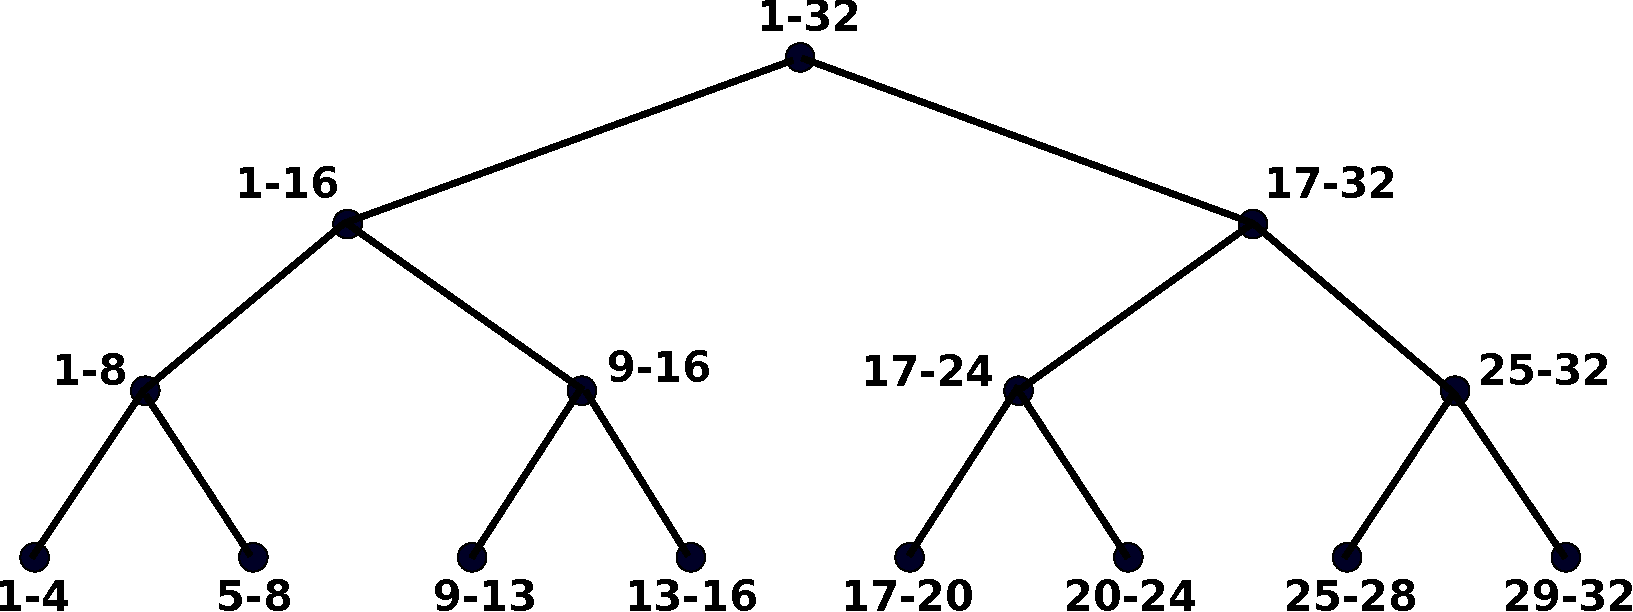
\includegraphics[width=0.7\linewidth]{chapters/4_hierarchical_matrices/figures/index_tree.pdf}
    \caption[Index Tree]{Example of a binary index tree over the index range 1-32. The resulting (sub-) ranges for each node are written next to it.}
    \label{fig:index_tree}
\end{figure}

The children in such a tree are usually ordered, so that the child holding the first part of the range of the parent will be number $1$ and the child holding the last part have number $c$ (where $c$ is the number of children). In the example this will correspond to the left child ($\#1$) and the right child ($\#2$) of a parent node. The root node in the graphic contains the full index set, which is then split equally in half by its children. This process is repeated recursively until a set of eight leaf nodes is obtained, each holding a subset of four indices. From left to right, those leaf nodes represent the full range of the root node.



\subsection{Cluster Tree}
\label{sec:cluster_tree}

The tensor product $\mathcal{T}$ of two index trees $\mathcal{I}$ and $\mathcal{J}$ represents a cluster tree, which can be described as a simple combination of the two index trees. The root of the cluster tree $\mathcal{T}$ contains both root nodes from $\mathcal{I}$ and $\mathcal{J}$. Each child node in $\mathcal{T}$ then holds a unique combination of children from $\mathcal{I}$ and $\mathcal{J}$ that are contained within its parent node. In other words, if $\mathcal{I}$ and $\mathcal{J}$ are binary index trees and the children of the root node are given by $\{I\#1, I\#2\}$ and $\{J\#1, J\#2\}$, the root node of $\mathcal{T}$ will have exactly four children, containing the pairings $\{I\#1, J\#1\}$, $\{I\#1, J\#2\}$, $\{I\#2, J\#1\}$ and $\{I\#2, J\#2\}$.

If both the nodes from $\mathcal{I}$ and $\mathcal{J}$ are leaf nodes, the node in $\mathcal{T}$ will also be a leaf. If only one of them is a leaf node, then the number of children of the node in $\mathcal{T}$ will be equal to the number of children from the internal node in $\mathcal{I}$ or $\mathcal{J}$. This is best discussed on the example depicted in Figure~\hyperref[fig:cluster_tree]{\ref{fig:cluster_tree}}. Suppose that the index ranges denoted in black correspond to the index tree $\mathcal{I}$, while the grey ones correspond to $\mathcal{J}$. Both are binary trees over the range 1-32, but $\mathcal{I}$ has a leaf size of 8 (i.e. three levels), while $\mathcal{J}$ has a leaf size of 16 (i.e. two levels). The root node spans the complete range of $32 \times 32$ and, due to the binary nature of the index trees, has four children. Each of these children holds an internal node from $\mathcal{I}$ and a leaf node from $\mathcal{J}$. Thus, these child nodes have two children each (the same as the number of children in $\mathcal{I}$), which will be the leaves of $\mathcal{T}$. Those leaf nodes hold one of the children from their parent node in $\mathcal{I}$ each, and the same node from $\mathcal{J}$ as their parent (since those are already leaf nodes). A mathematically rigorous definition and analysis of such cluster trees can be obtained from \cite{hackbusch_hierarchical_2015}

\begin{figure}[h]
    \centering
    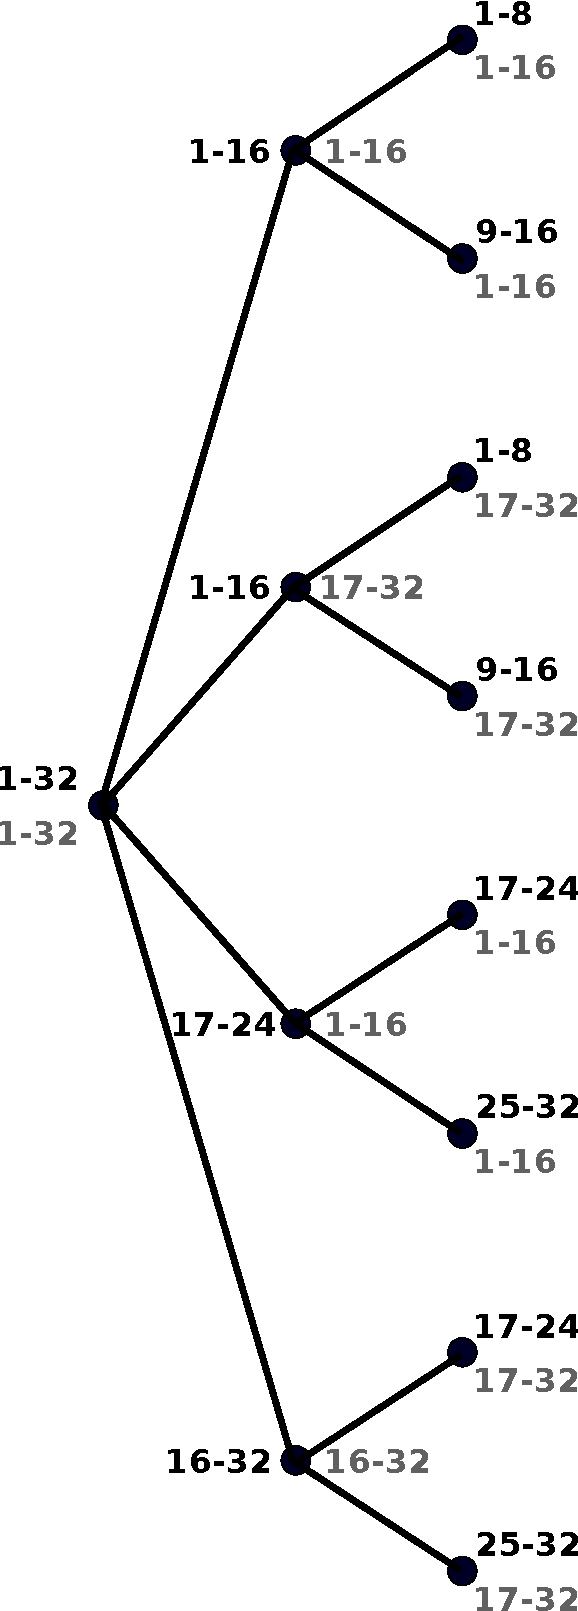
\includegraphics[width=0.3\linewidth]{chapters/4_hierarchical_matrices/figures/cluster_tree.pdf}
    \caption[Cluster Tree]{Example of a cluster tree from two index trees with a range of 1-32. The ranges for the index tree $\mathcal{I}$ are denoted in black, while those of $\mathcal{J}$ are grey.}  \label{fig:cluster_tree}
\end{figure}